\documentclass[11pt]{article}
\usepackage[margin=1in]{geometry}
\usepackage{amsmath,amssymb,amsthm}
\usepackage{graphicx}
\usepackage{microtype}
\usepackage[hidelinks]{hyperref}

\newtheorem{theorem}{Theorem}
\newtheorem{lemma}{Lemma}
\newcommand{\cO}{\mathcal O}

\title{Complete Saturation of the Natural Operator Space $O\ell_p$\\
\large A candidate affirmative solution to Question 4.13 of arXiv:1704.07760}
\author{Automated mathematical discovery run \texttt{fa\_banach\_001}, lane 15}
\date{11 August 2026}

\begin{document}
\maketitle

\begin{center}
\fbox{\parbox{0.91\linewidth}{\textbf{Status.} Candidate full solution,
likely valid, requiring expert review. A bounded search found no explicit
later resolution.}}
\end{center}

\begin{abstract}
We answer Question 4.13 of Corr\^ea affirmatively. In fact, for every
$1\leq p<\infty$, including $p=2$, the natural operator space $O\ell_p$ is
$O\ell_p$-completely saturated. Every infinite-dimensional subspace of
$\ell_p$ contains a normalized sequence summably close to a normalized
disjoint block sequence. Disjoint normalized sequences are completely
isometric to the canonical basis in the natural operator $L_p$ structure,
and a summable perturbation is small in completely bounded norm because it
is a sum of rank-one maps. Choosing the total error below one completes the
argument.
\end{abstract}

\section{Source question}

Corr\^ea equips $\ell_p$ with its natural operator-space structure
$O\ell_p=(\min\ell_\infty,\max\ell_1)_{1/p}$ and asks whether it is
$O\ell_p$-completely saturated \cite{source}.

\begin{figure}[ht]
  \centering
  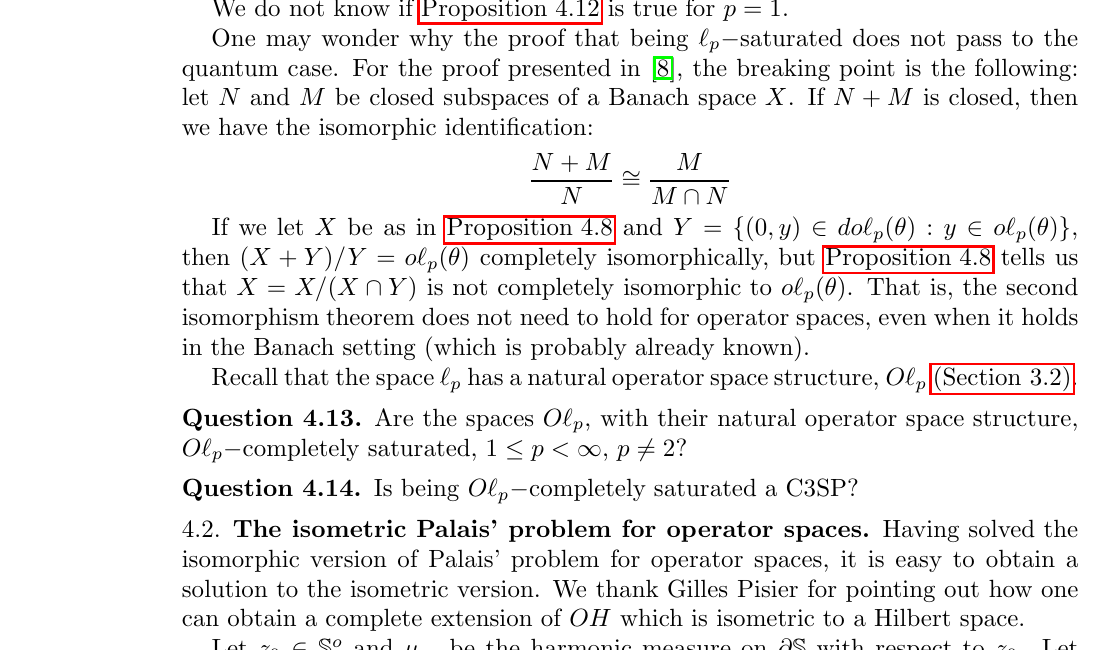
\includegraphics[width=0.96\linewidth]{figures/question_4_13_crop.png}
  \caption{Question 4.13 and its context in the source, PDF p.~29.}
\end{figure}

Recall that an operator space $E$ is $E$-completely saturated when every
closed infinite-dimensional subspace contains a subspace completely
isomorphic to $E$.

\section{Two lemmas}

We use the standard natural operator-space structure on the commutative
$L_p$-space $\ell_p$. Its complete Fubini identity is
\begin{equation}\label{eq:fubini}
 S_p^n[O\ell_p]\cong \ell_p(S_p^n)
\end{equation}
isometrically. A map between operator spaces is a complete isometry if and
only if all its $S_p^n$-amplifications are isometries \cite{pisier}.

\begin{lemma}\label{lem:disjoint}
Let $(u_k)$ be a disjointly supported sequence in $\ell_p$ with
$\|u_k\|_p=1$. The map $V:O\ell_p\to O\ell_p$ defined by
$V(e_k)=u_k$ is a complete isometry onto its range.
\end{lemma}

\begin{proof}
For a finite family $A_k\in S_p^n$, \eqref{eq:fubini} and disjointness give
\begin{align*}
 \left\|\sum_k A_k\otimes u_k\right\|_{S_p^n[O\ell_p]}^p
 &=\sum_j\left\|\sum_k u_k(j)A_k\right\|_{S_p^n}^p\\
 &=\sum_k\sum_{j\in\operatorname{supp}u_k}
        |u_k(j)|^p\|A_k\|_{S_p^n}^p
 =\sum_k\|A_k\|_{S_p^n}^p.
\end{align*}
The last expression is the norm of $\sum_k A_k\otimes e_k$ to the
$p$-th power. The amplification criterion proves the claim.
\end{proof}

\begin{lemma}\label{lem:perturb}
If $(d_k)\subset O\ell_p$ and $\sum_k\|d_k\|_p=\eta<\infty$, then
$D(e_k)=d_k$ extends to a completely bounded map on $O\ell_p$ with
$\|D\|_{cb}\leq\eta$. Consequently, if $V$ is a complete isometry and
$\eta<1$, then $V+D$ is a complete isomorphism onto a closed range.
\end{lemma}

\begin{proof}
Let $e_k^*$ be the $k$-th coordinate functional. Every bounded scalar-valued
functional on an operator space has the same norm and cb norm, and the map
$\lambda\mapsto\lambda d_k$ has cb norm $\|d_k\|_p$. Thus
\[
 D=\sum_k e_k^*\otimes d_k
\]
converges absolutely in cb norm and $\|D\|_{cb}\leq\eta$. At every matrix
level,
\[
 (1-\eta)\|z\|\leq\|(V+D)_n z\|\leq(1+\eta)\|z\|.
\]
This gives a complete isomorphism and a closed range.
\end{proof}

\section{Affirmative solution}

\begin{theorem}\label{thm:main}
For every $1\leq p<\infty$, the natural operator space $O\ell_p$ is
$O\ell_p$-completely saturated. In particular, Question 4.13 of
\cite{source} has an affirmative answer.
\end{theorem}

\begin{proof}
Let $W$ be a closed infinite-dimensional subspace of $\ell_p$. Fix positive
numbers $(\delta_k)$ such that $2\sum_k\delta_k<1$. We inductively construct
integers
\[
 0=N_0<N_1<N_2<\cdots
\]
and unit vectors $x_k\in W$. The restriction to $W$ of the projection onto
the first $N_{k-1}$ coordinates has finite rank, so its kernel is
infinite-dimensional. Choose $x_k$ in that kernel with $\|x_k\|_p=1$, and
then choose $N_k$ so that
\[
 \left\|x_k-P_{(N_{k-1},N_k]}x_k\right\|_p<\delta_k.
\]

Put $v_k=P_{(N_{k-1},N_k]}x_k$ and $u_k=v_k/\|v_k\|_p$. The vectors $u_k$
are normalized and disjointly supported. Moreover,
\[
 \|x_k-u_k\|_p
 \leq \|x_k-v_k\|_p+|1-\|v_k\|_p|
 <2\delta_k.
\]
By Lemma \ref{lem:disjoint}, $V(e_k)=u_k$ is a complete isometry. By Lemma
\ref{lem:perturb}, the map $D(e_k)=x_k-u_k$ satisfies
\[
 \|D\|_{cb}\leq\sum_k\|x_k-u_k\|_p
 <2\sum_k\delta_k<1.
\]
Hence $U=V+D$ is a complete isomorphism from $O\ell_p$ onto the closed span
of $(x_k)$. Since every $x_k$ belongs to $W$, this closed span is contained
in $W$. The arbitrary infinite-dimensional subspace $W$ therefore contains
a completely isomorphic copy of $O\ell_p$.
\end{proof}

\section{Verification and novelty bounds}

The proof audit checks the gliding-hump construction, the factor two caused
by normalizing the block vectors, the complete Fubini calculation, absolute
cb-norm convergence of the rank-one perturbations, and the matrix-level
lower bound for $V+D$. No finite computation is relevant.

The conclusion addresses complete saturation only. It does not answer the
source's subsequent Question 4.14 asking whether this property is a complete
three-space property.

A bounded search on 11 August 2026 covered the run's registry, solution,
attempt, and active-claim indexes; the exact arXiv id and title; exact phrases
from Question 4.13; combinations of $O\ell_p$, operator spaces, and complete
saturation; published-paper metadata; and later citations of the source. No
explicit answer was located. This is provisional novelty evidence only.

\section*{Human-review recommendation}

Check first the complete Fubini identity \eqref{eq:fubini} and the standard
$S_p$ amplification criterion. Then verify that the coordinate rank-one
series converges in cb norm. The gliding-hump part is the usual elementary
coordinate argument in $\ell_p$ and includes $p=1$ without a weak-nullness
assumption.

\begin{thebibliography}{9}
\bibitem{source}
W. H. G. Corr\^ea,
\emph{Twisting Operator Spaces}, Trans. Amer. Math. Soc. \textbf{370}
(2018), 8921--8957; arXiv:1704.07760, Question 4.13.

\bibitem{pisier}
G. Pisier,
\emph{Introduction to Operator Space Theory}, Cambridge University Press,
2003; see the natural operator $L_p$ structure, complete Fubini, and the
$S_p$ amplification criterion.
\end{thebibliography}

\end{document}
